\documentclass[simplex.tex]{subfiles}
% NO NEED TO INPUT PREAMBLES HERE
% packages are inherited; you can compile this on its own
\begin{document}
\subsection[meda]{meda \href{https://github.com/mrae}{@JesseLP}}

Updates in \href{https://github.com/neurodata/meda}{meda} include the
addition of plots that explore the clusters generated by
hierarchical clustering.  We are using 
\href{http://www.stat.washington.edu/fraley/mclust/}{mclust}~ \citereferences{fraley2002} 
in our
hierarchical clustering function.  At each level we use the Bayseian
Information Criterion (BIC) to determine if the data should be split
into two clusters or kept as one.  The dendrogram 
(figure \ref{fig:meda}~left)
shows the binary tree clustering structure with branch size denoting the
size of the cluster.  The stacked level means plot
(figure \ref{fig:meda}~right) shows the means of features in each node 
of the tree.


\begin{figure}[!h]
\begin{cframed}
\centering
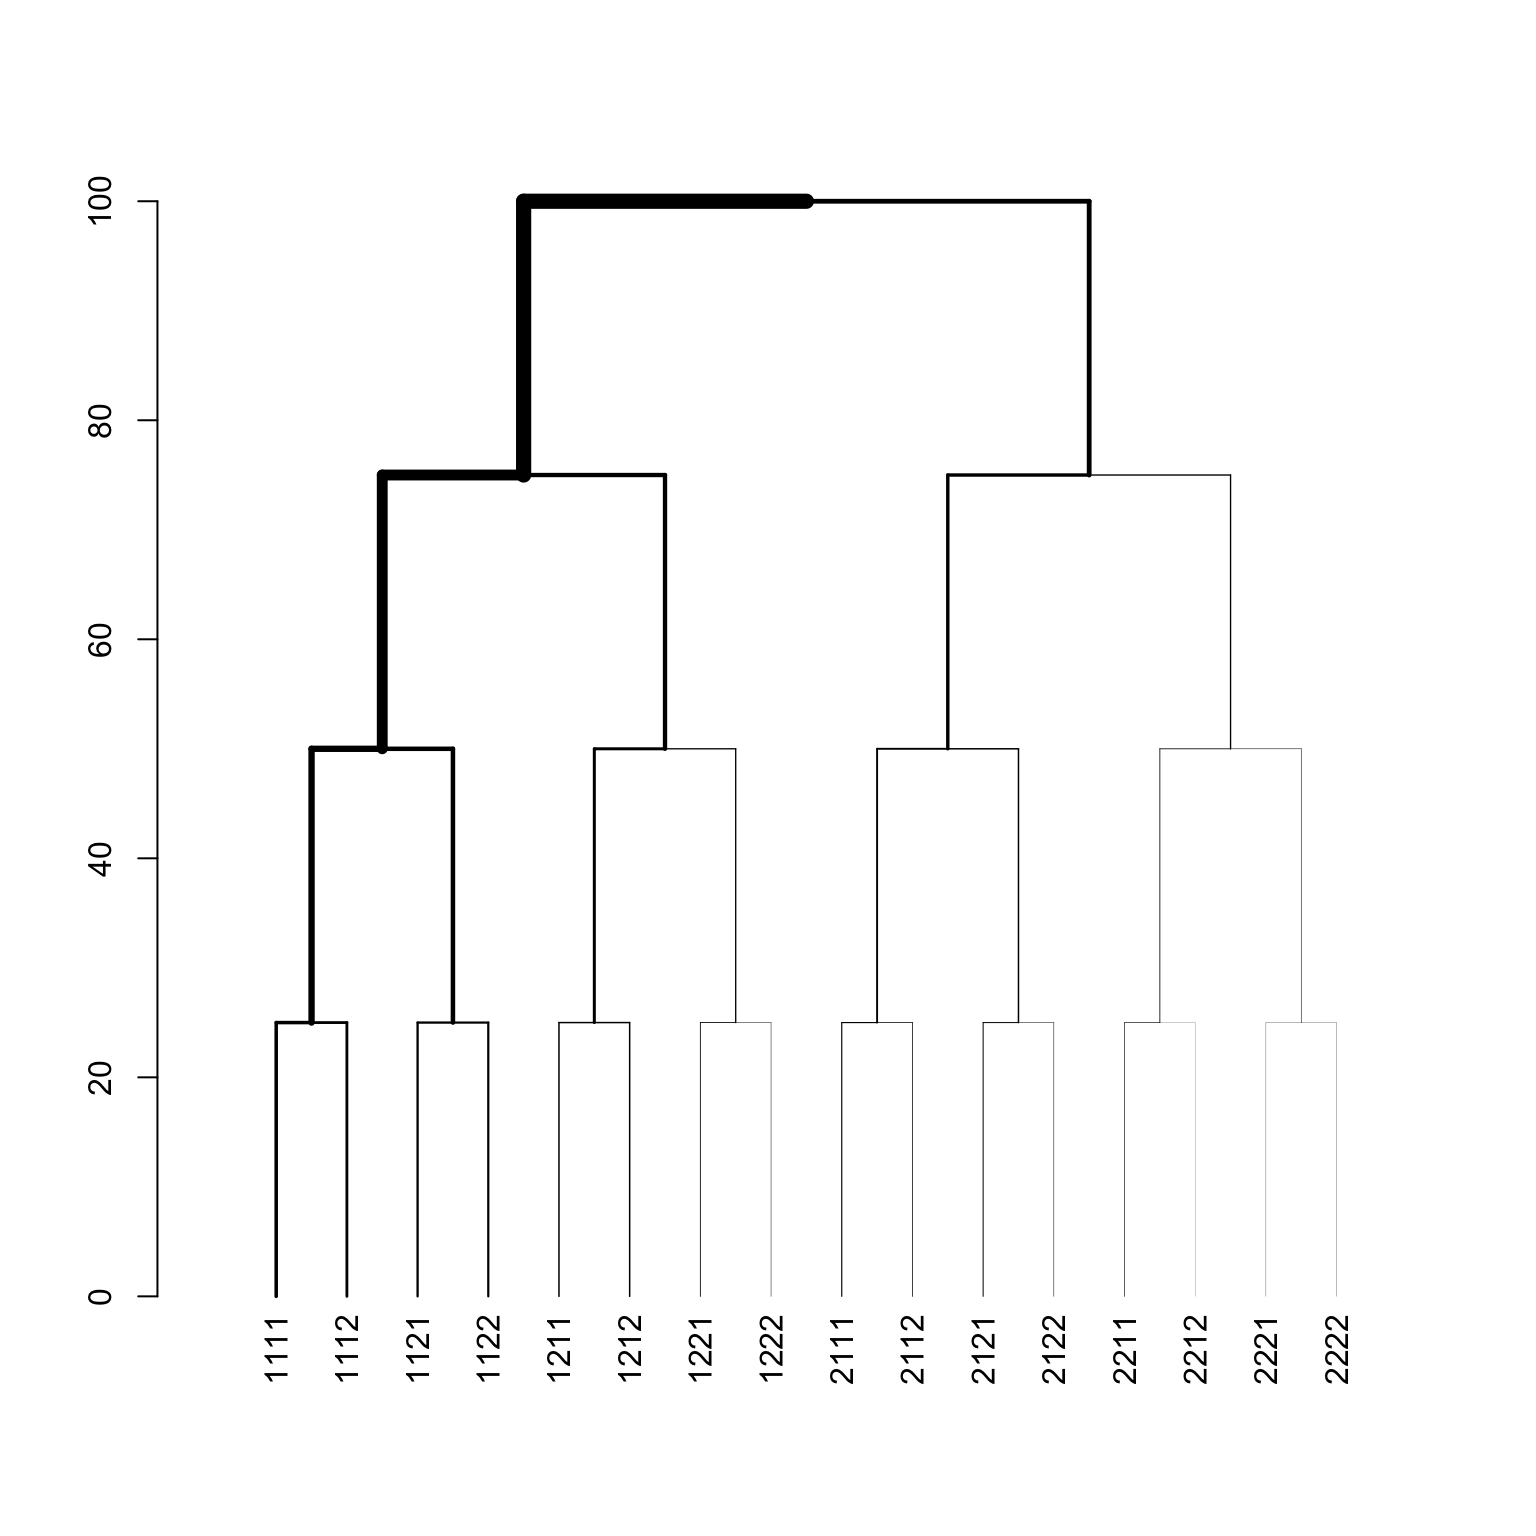
\includegraphics[width=0.45\textwidth, clip = true, trim = 2cm 5cm 4cm 6cm ]{../../figs/K15_samp1e4_01e3_dendro.png}
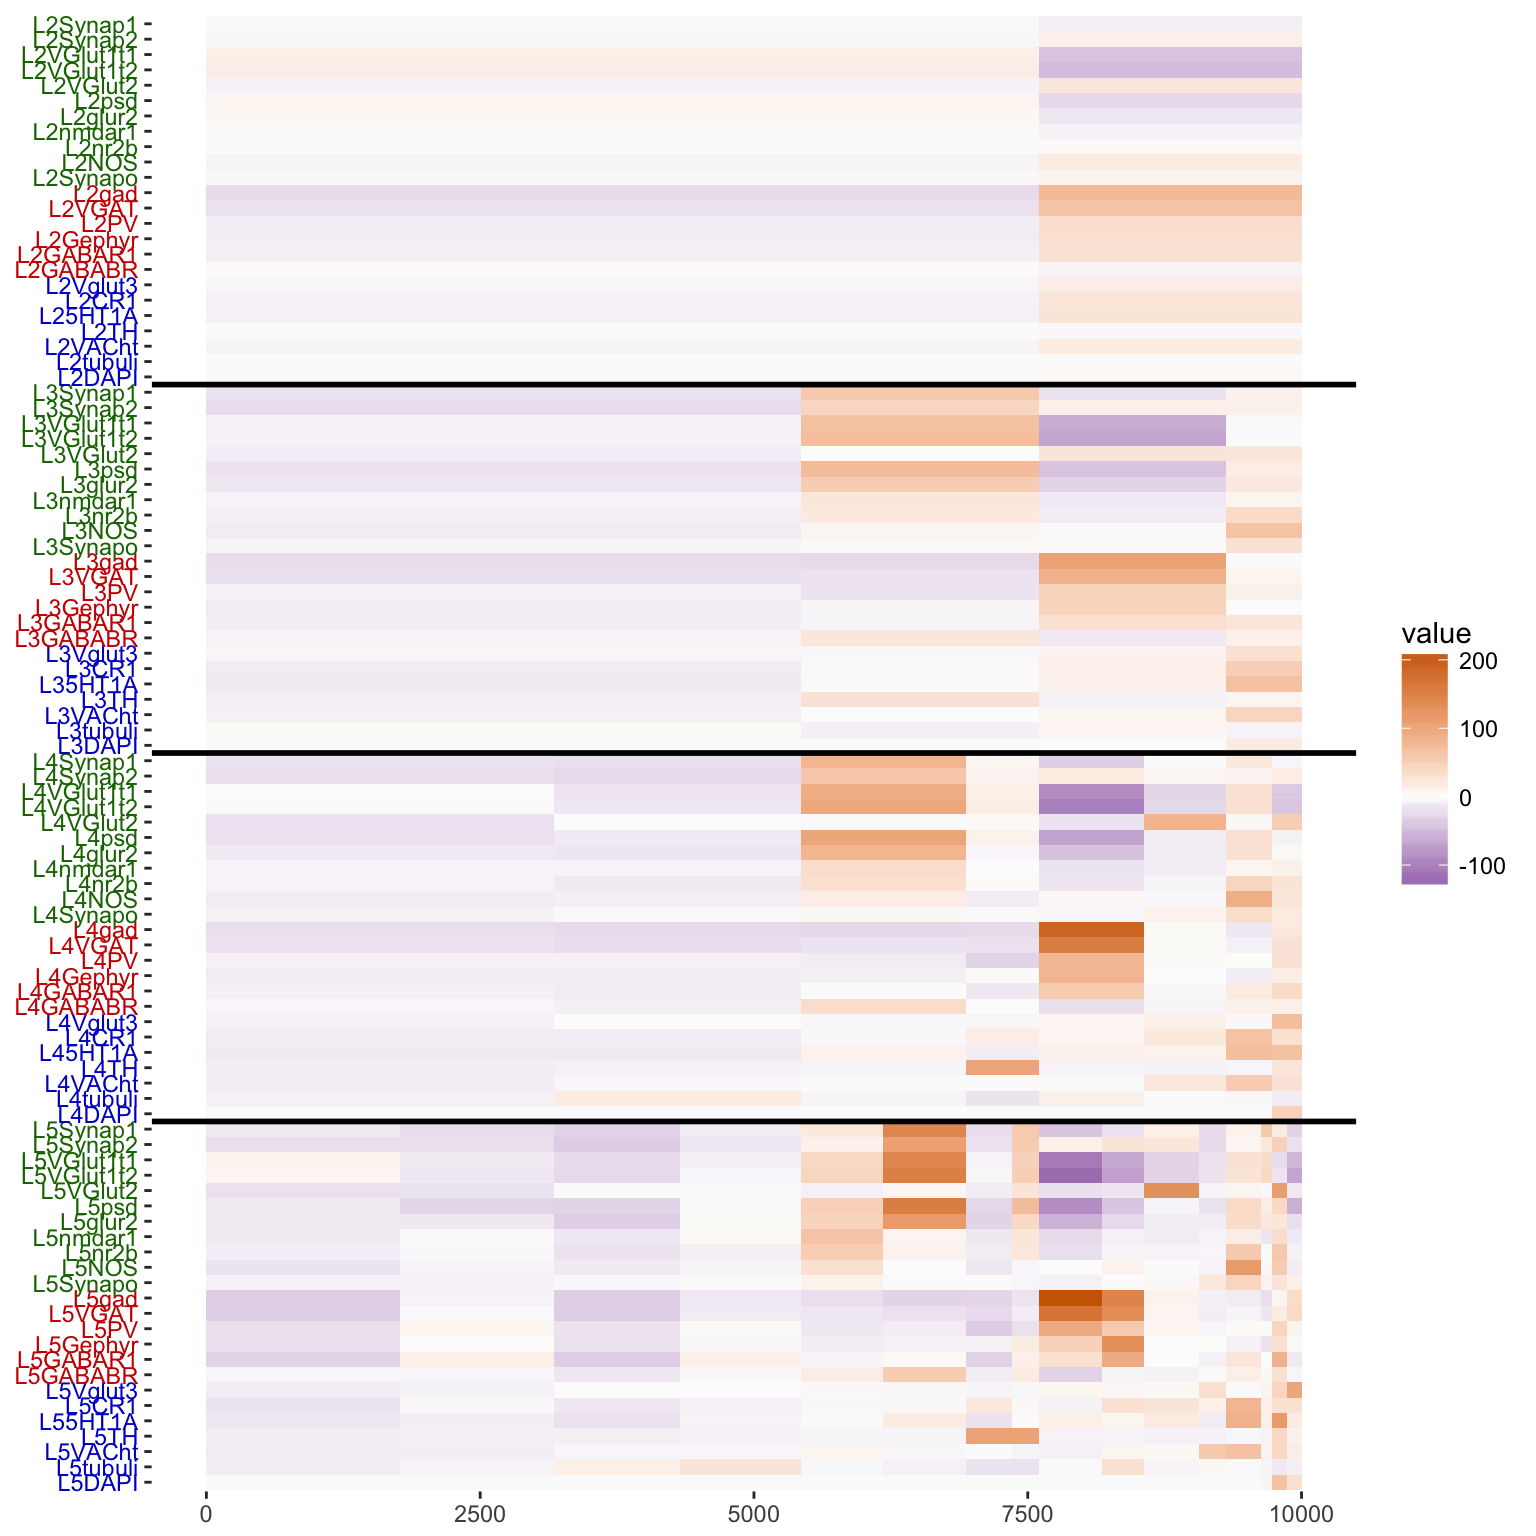
\includegraphics[width=0.45\textwidth, clip = true, trim = 1cm 0 5mm 1mm]{../../figs/K15_samp1e4_01e3_slcmeans.png}
\caption{Left:  A dendrogram showing the results of hierarchical mclust.
The splits are constrained to be binary and branch sizes show relative
cluster sizes.  Right: A stacked level means plot showing for each node
in the dendrogram the feature means.}
\label{fig:meda}
\end{cframed}
\end{figure}

\clearpage
\end{document}
